\chapter{Oscillators, Occupation Numbers, and the First Quantum Field}

These notes follow Leonard Susskind's sixth lecture in \emph{Advanced Quantum Mechanics}, curated by LazyingArt LLC (\texttt{https://lazying.art}). The lecture enters quantum field theory in the gentlest possible way. Rather than beginning with relativistic formalism, Susskind first returns to the harmonic oscillator and insists that its operator algebra is the real prerequisite for second quantization. From there the lecture proceeds in a carefully staged order: a single oscillator, many oscillators, occupation numbers, one-particle states in a box, and finally the operator-valued field \(\Psi(x)\) that creates and annihilates particles at a point.

\section{Why Harmonic Oscillators Come First}

Susskind opens by reminding us why quantum field theory matters: apart from gravity, it is the framework in which modern fundamental physics is written. But he immediately narrows the scope. The full subject is too complicated to attack head-on, so the lecture begins with the most elementary mathematical structure that later survives intact inside field theory.

The crucial point is that when he says \emph{harmonic oscillator}, he no longer means a spring in the usual mechanical sense. He means the algebra of a pair of adjoint operators, one that raises an excitation level and one that lowers it, together with the number operator built from them. This is the mathematical core that will later be reinterpreted as particle creation and annihilation.

We will write these operators as \(a^\dagger\) and \(a\), even though the lecture begins with the notation \(A_+\) and \(A_-\). The change is only notational. The content is the same.

\section{Single-Oscillator Algebra and Energy Quanta}

For a single oscillator, the basic data are
\begin{align}
a|0\rangle &= 0, \\
N &= a^\dagger a, \\
N|n\rangle &= n|n\rangle, \\
[a,a^\dagger] &= 1.
\end{align}
The state \(|0\rangle\) is the lowest state, and the states \(|n\rangle\) are eigenstates of the number operator \(N\).

\begin{remark}
Susskind briefly recalls that \(a^\dagger\) and \(a\) can be expressed in terms of \(x\) and \(p\), but the lecture immediately shifts to the algebraic viewpoint. Since the spoken formulas are hesitant and partly self-corrected, it is cleaner here to emphasize the algebra rather than a specific convention for \(x\) and \(p\).
\end{remark}

The Hamiltonian of the oscillator is, up to the usual zero-point term,
\begin{equation}
H = \hbar \omega \left(N+\frac{1}{2}\right).
\end{equation}
In this lecture the additive constant \(\frac{1}{2}\hbar\omega\) is set aside, because the emphasis is on the spacing between levels:
\begin{equation}
H_{\mathrm{free}} = \hbar \omega N.
\end{equation}
The physical meaning is simple and important. Every time the occupation number increases by one unit, the energy increases by one quantum \(\hbar\omega\). Every time it decreases by one unit, the system releases that same amount of energy.

This is already the first hint of field theory. The number operator counts excitations, and the cost of one additional excitation is fixed by the frequency.

\section{Many Oscillators and Occupation Numbers}

The next step is to consider many independent oscillators, labeled by an index \(i\). Susskind insists on the reason for the algebra: independent subsystems must be described by commuting operators, for otherwise they could not be measured independently. This immediately leads to the multimode relations
\begin{equation}
[a_i,a_j]=0,\qquad [a_i^\dagger,a_j^\dagger]=0,\qquad [a_i,a_j^\dagger]=\delta_{ij}.
\end{equation}
For each mode there is a number operator
\begin{equation}
N_i = a_i^\dagger a_i,
\end{equation}
and the free Hamiltonian is the sum of the energies of all modes,
\begin{equation}
H = \sum_i \hbar \omega_i N_i.
\end{equation}
Later in the lecture Susskind drops \(\hbar\) and writes the same formula as
\begin{equation}
H = \sum_i \omega_i a_i^\dagger a_i.
\end{equation}

A basis of states is now specified by listing the occupation number of every mode:
\begin{equation}
|n_1,n_2,n_3,\ldots\rangle.
\end{equation}
The integer \(n_i\) is the occupation number of the \(i\)-th oscillator. At this stage it is only a name, but the lecture soon turns that name into a particle interpretation.

The vacuum in this language is the state with zero occupation in every mode,
\begin{equation}
|0\rangle = |0,0,0,\ldots\rangle,
\end{equation}
and it is characterized by
\begin{equation}
a_i|0\rangle = 0 \qquad \text{for all } i.
\end{equation}

\section{Deriving the Ladder Coefficients}

Up to this point the raising and lowering rules have been schematic. Susskind then pauses for a real derivation. The issue is that if the number states are normalized, the action of \(a^\dagger\) on \(|n\rangle\) cannot simply be \(|n+1\rangle\). There must be a numerical coefficient.

Start with the ansatz
\begin{equation}
a^\dagger |n\rangle = c_n |n+1\rangle.
\end{equation}
This is the step clearly visible on the board. The coefficient \(c_n\) is to be determined from the commutation relations and the normalization of the states.

\begin{proposition}
For normalized number states,
\begin{equation}
a^\dagger |n\rangle = \sqrt{n+1}\,|n+1\rangle,
\qquad
a|n\rangle = \sqrt{n}\,|n-1\rangle.
\end{equation}
\end{proposition}

\begin{proof}
Take the Hermitian conjugate of the ansatz:
\begin{equation}
\langle n|a = c_n \langle n+1|,
\end{equation}
where, as in the lecture, \(c_n\) is chosen real for simplicity.

Now multiply the bra equation by the ket equation:
\begin{equation}
\langle n|aa^\dagger|n\rangle = c_n^2 \langle n+1|n+1\rangle.
\end{equation}
Because the states are normalized, \(\langle n+1|n+1\rangle=1\), so
\begin{equation}
\langle n|aa^\dagger|n\rangle = c_n^2.
\end{equation}
Using the commutator,
\begin{equation}
aa^\dagger = a^\dagger a + 1 = N+1.
\end{equation}
Therefore
\begin{equation}
c_n^2 = \langle n|(N+1)|n\rangle = n+1,
\end{equation}
and hence
\begin{equation}
c_n = \sqrt{n+1}.
\end{equation}
This proves
\begin{equation}
a^\dagger|n\rangle = \sqrt{n+1}\,|n+1\rangle.
\end{equation}

The lowering rule is derived in the same way, and gives
\begin{equation}
a|n\rangle = \sqrt{n}\,|n-1\rangle.
\end{equation}
At \(n=0\) this automatically yields \(a|0\rangle=0\).
\end{proof}

The importance of the square roots is partly algebraic and partly interpretive. Algebraically, they are what make the normalized states transform correctly under \(a^\dagger a\). Physically, Susskind emphasizes that sometimes the coefficient has no separate tangible meaning beyond ensuring the internal consistency of the quantum-mechanical normalization.

For many oscillators, the same rule acts one slot at a time:
\begin{align}
a_i^\dagger |n_1,\ldots,n_i,\ldots\rangle
&=
\sqrt{n_i+1}\,|n_1,\ldots,n_i+1,\ldots\rangle, \\
a_i |n_1,\ldots,n_i,\ldots\rangle
&=
\sqrt{n_i}\,|n_1,\ldots,n_i-1,\ldots\rangle.
\end{align}
All other occupation numbers are spectators.

\section{One-Particle States in a Box}

Only after the oscillator algebra is fully in place does Susskind turn back to the connection between particles and fields. He first explains what a familiar wavefunction \(\psi\) is and what it is not.

For one particle, \(\psi(x)\) is the state vector in the position representation. It is not itself an observable. For several particles, the wavefunction is no longer a function of one position but of all particle positions,
\begin{equation}
\psi(x_1,\ldots,x_N).
\end{equation}
Most importantly, such a wavefunction describes a \emph{fixed} number of particles. That, Susskind says, is not yet the idea of a quantum field.

To build the bridge, he returns to ordinary one-particle quantum mechanics and chooses a particle in a box. The one-particle energy eigenstates are wavefunctions
\begin{equation}
\psi_1(x),\ \psi_2(x),\ \psi_3(x),\ \ldots
\end{equation}
arranged in order of increasing energy. The lecture only needs their qualitative form: the lowest mode is the smoothest one that fits in the box, the next has one node, and higher modes oscillate more rapidly. If one wants a standard explicit model for an ideal infinite box of length \(L\), one may take
\begin{equation}
\psi_n(x)=\sqrt{\frac{2}{L}}\sin\!\left(\frac{n\pi x}{L}\right),
\qquad 0<x<L,
\end{equation}
but the lecture itself uses only the ordered family of orthonormal one-particle states.

\begin{figure}[ht]
\centering
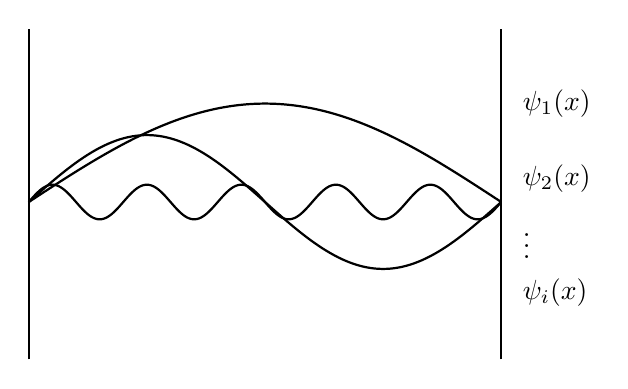
\begin{tikzpicture}[x=1cm,y=1cm]
\draw[thick] (0,0) -- (0,4.2);
\draw[thick] (6,0) -- (6,4.2);

\draw[thick,domain=0:6,samples=120] plot (\x,{2+1.25*sin(180*\x/6)});
\draw[thick,domain=0:6,samples=120] plot (\x,{2+0.85*sin(360*\x/6)});
\draw[thick,domain=0:6,samples=240] plot (\x,{2+0.22*sin(1800*\x/6)});

\node[right] at (6.15,3.25) {$\psi_1(x)$};
\node[right] at (6.15,2.30) {$\psi_2(x)$};
\node[right] at (6.15,1.55) {$\vdots$};
\node[right] at (6.15,0.85) {$\psi_i(x)$};
\end{tikzpicture}
\caption{Qualitative one-particle basis functions in a one-dimensional box, following the lecture's board sketch. The node structure and ordering matter more than the precise amplitudes.}
\end{figure}

Now comes the key reinterpretation. Suppose there are many bosons, of undetermined total number, occupying these one-particle states. Then a basis of many-body states is specified by saying how many particles occupy each one-particle mode:
\begin{equation}
|n_1,n_2,n_3,\ldots\rangle.
\end{equation}
This is exactly the same occupation-number notation that described many oscillators. The coincidence is the point. The many-boson system can be organized as if each one-particle state were its own oscillator.

The free Hamiltonian becomes
\begin{equation}
H = \sum_i \omega_i a_i^\dagger a_i.
\end{equation}
Here \(\omega_i\) is the energy of the \(i\)-th one-particle state, after Susskind has dropped \(\hbar\). An important clarification from the discussion after the break is that the \(\omega_i\) need not be evenly spaced. The one-particle energy levels in a box are not harmonic-oscillator levels. What is evenly spaced is the ladder of occupation numbers for each \emph{fixed} mode: zero particles, one particle, two particles, and so on.

Throughout this lecture the particles are free, meaning non-interacting. That is why the total energy is simply additive over the occupied one-particle states.

\section{The Nonrelativistic Field Operator}

We are now ready for the central definition. A quantum field is not merely a wavefunction. It is an operator on the variable-particle-number state space, and it depends on one spatial point. In the present nonrelativistic bosonic setting, Susskind defines
\begin{equation}
\Psi(x)=\sum_i a_i\,\psi_i(x).
\end{equation}
Its Hermitian conjugate is
\begin{equation}
\Psi^\dagger(x)=\sum_i a_i^\dagger\,\psi_i^*(x).
\end{equation}
The functions \(\psi_i(x)\) are ordinary complex numbers once \(x\) is specified; the operator character sits entirely in the \(a_i\) and \(a_i^\dagger\).

This is also the point at which the Fourier analogy becomes visible. If the \(\psi_i\) are chosen as momentum eigenfunctions, then the \(a_i\) play the role of quantum-mechanical Fourier coefficients. More generally, the definition works for any orthonormal one-particle basis.

\begin{remark}
Susskind first motivates \(\Psi\) as the kind of object one wants to measure, but later emphasizes that \(\Psi\) and \(\Psi^\dagger\) are not Hermitian. The right conclusion is that \(\Psi\) is an operator-valued field, while Hermitian combinations such as \(\Psi+\Psi^\dagger\) are the directly observable combinations.
\end{remark}

\subsection{Action on the Vacuum}

The crucial calculation is to show what \(\Psi^\dagger(x)\) does to the vacuum. Let \(|i\rangle\) denote the one-particle state whose wavefunction is \(\psi_i(x)\), with
\begin{equation}
\langle x|i\rangle = \psi_i(x).
\end{equation}
Completeness of the one-particle basis gives
\begin{equation}
\sum_i |i\rangle\langle i| = 1.
\end{equation}
Apply this to the position eigenstate \(|x\rangle\):
\begin{align}
|x\rangle
&=
\sum_i |i\rangle\langle i|x\rangle \\
&=
\sum_i \psi_i^*(x)\,|i\rangle.
\end{align}
But a one-particle state \(|i\rangle\) is created from the vacuum by
\begin{equation}
|i\rangle = a_i^\dagger |0\rangle.
\end{equation}
Therefore
\begin{align}
|x\rangle
&=
\sum_i \psi_i^*(x)\,a_i^\dagger |0\rangle \\
&=
\Psi^\dagger(x)|0\rangle.
\end{align}
So \(\Psi^\dagger(x)\) creates a particle at position \(x\).

By contrast,
\begin{equation}
\Psi(x)|0\rangle = 0,
\end{equation}
because every term in \(\Psi(x)\) contains an annihilation operator.

\subsection{Vacuum Versus the Zero Vector}

Susskind spends a long stretch of the lecture clearing up a common confusion. The vacuum \(|0\rangle\) is not the zero vector. It is a perfectly good normalized state, the state of empty space in this simplified setting. The symbol \(0\) in \(|0\rangle\) is only a label: it means zero particles, not zero norm.

When an annihilation operator hits the vacuum, the result is the genuine zero vector,
\begin{equation}
a_i|0\rangle = 0.
\end{equation}
That vector has zero length and cannot be normalized. It is not a physical state. This distinction matters whenever one interprets the statement that an annihilation operator ``gives zero.'' It does not return the vacuum; it returns the zero vector.

\subsection{Two Particles and Bosonic Symmetry}

Once \(\Psi^\dagger(x)\) is understood as the operator that inserts a particle at \(x\), the natural two-particle state is
\begin{equation}
\Psi^\dagger(y)\Psi^\dagger(x)|0\rangle.
\end{equation}
Expanding both fields,
\begin{equation}
\Psi^\dagger(y)\Psi^\dagger(x)
=
\sum_{i,j} a_i^\dagger a_j^\dagger \,\psi_i^*(y)\psi_j^*(x).
\end{equation}
Because the creation operators commute for bosons,
\begin{equation}
[a_i^\dagger,a_j^\dagger]=0,
\end{equation}
it follows that
\begin{equation}
\Psi^\dagger(y)\Psi^\dagger(x)|0\rangle
=
\Psi^\dagger(x)\Psi^\dagger(y)|0\rangle.
\end{equation}
Thus the state is symmetric under exchange of \(x\) and \(y\). In the lecture this is the moment when bosonic statistics emerges directly from the operator construction.

A single field of this type describes a single species of boson. Different species require different fields. In that sense the field carries the information about \emph{what kind} of particle is being created, while the spatial argument \(x\) specifies \emph{where} it is created.

\section{Summary}

The lecture reaches quantum field theory by a sequence of controlled reinterpretations. First, the harmonic oscillator is reduced to its operator algebra. Next, many independent oscillators are organized by occupation numbers. Then one-particle energy eigenstates in a box are re-read as modes that can be occupied by any number of bosons. Finally, the field operator
\begin{equation}
\Psi(x)=\sum_i a_i\psi_i(x)
\end{equation}
packages those creation and annihilation operators into an operator attached to each point in space.

The conceptual payoff is large. A fixed-particle-number wavefunction \(\psi(x_1,\ldots,x_N)\) is replaced by a framework that can describe zero particles, one particle, two particles, or a superposition of all of them. In Susskind's language, quantum field theory is at least a bookkeeping device for variable particle number; in more physical language, it is the operator formalism in which particles are understood as quanta of fields. In this nonrelativistic bosonic example, that whole structure is already visible.